\documentclass[11pt,oneside]{article}

\usepackage[a4paper,margin=25mm,headheight=15pt]{geometry}
\usepackage[T1]{fontenc}
\usepackage[utf8]{inputenc}
\IfFileExists{libertinus.sty}{\usepackage{libertinus}}{\usepackage{lmodern}}
\usepackage{microtype}
\usepackage{amsmath,amssymb,amsthm,mathtools,mathrsfs,bm}
\usepackage{booktabs,longtable,tabularx,array}
\usepackage{graphicx}
\usepackage{float}
\usepackage{xcolor}
\usepackage{enumitem}
\usepackage{fancyhdr}
\usepackage{titlesec}
\usepackage{xurl}
\usepackage{listings}
\usepackage[most]{tcolorbox}
\usepackage[hypertexnames=false]{hyperref}
\usepackage[nameinlink,noabbrev]{cleveref}

\definecolor{linkblue}{RGB}{30,76,130}
\definecolor{deepgreen}{RGB}{28,104,74}
\definecolor{shadegray}{RGB}{247,248,250}
\definecolor{rulegray}{RGB}{194,201,210}
\hypersetup{
  colorlinks=true,
  linkcolor=linkblue,
  citecolor=deepgreen,
  urlcolor=linkblue,
  pdftitle={Complete Small-Argument Asymptotics of the Inverse Fabius Function},
  pdfauthor={Research report prepared for Vladimir Reshetnikov},
  pdfsubject={Arbitrary-order phase-aware inverse asymptotics, closed coefficient formulas, and a 2-adic Mellin bridge},
  pdfkeywords={Fabius function, inverse Fabius function, Lambert W, Bell polynomial, Lagrange inversion, Thue-Morse, 2-adic valuation, Mellin transform, asymptotic expansion}
}

\pagestyle{fancy}
\fancyhf{}
\fancyhead[L]{\small Inverse Fabius asymptotics}
\fancyhead[R]{\small Closed coefficients and dyadic sectors}
\fancyfoot[C]{\thepage}
\renewcommand{\headrulewidth}{0.4pt}
\titleformat{\section}{\Large\bfseries}{\thesection}{0.7em}{}
\titleformat{\subsection}{\large\bfseries}{\thesubsection}{0.7em}{}
\titleformat{\subsubsection}{\normalsize\bfseries}{\thesubsubsection}{0.7em}{}
\setcounter{secnumdepth}{3}
\setcounter{tocdepth}{2}
\setlist[itemize]{leftmargin=2em,itemsep=0.22em,topsep=0.35em}
\setlist[enumerate]{leftmargin=2.3em,itemsep=0.22em,topsep=0.35em}
\allowdisplaybreaks[2]
\numberwithin{equation}{section}
\setlength{\emergencystretch}{3em}

\newtheorem{theorem}{Theorem}[section]
\newtheorem{proposition}[theorem]{Proposition}
\newtheorem{lemma}[theorem]{Lemma}
\newtheorem{corollary}[theorem]{Corollary}
\newtheorem{conjecture}[theorem]{Conjecture}
\newtheorem{algorithm}[theorem]{Algorithm}
\theoremstyle{definition}
\newtheorem{definition}[theorem]{Definition}
\newtheorem{example}[theorem]{Example}
\newtheorem{obligation}[theorem]{Formalization obligation}
\theoremstyle{remark}
\newtheorem{remark}[theorem]{Remark}
\newtheorem{warning}[theorem]{Warning}

\newcommand{\R}{\mathbb R}
\newcommand{\C}{\mathbb C}
\newcommand{\N}{\mathbb N}
\newcommand{\Z}{\mathbb Z}
\newcommand{\Q}{\mathbb Q}
\newcommand{\E}{\mathbb E}
\newcommand{\Prob}{\mathbb P}
\newcommand{\e}{\mathrm e}
\newcommand{\ii}{\mathrm i}
\newcommand{\dd}{\,\mathrm d}
\newcommand{\bigO}{\mathcal O}
\newcommand{\smallo}{o}
\newcommand{\Res}{\operatorname{Res}}
\newcommand{\coeff}[2]{[#1^{#2}]}
\newcommand{\LambertW}{W}
\newcommand{\Up}{\operatorname{up}}
\newcommand{\abs}[1]{\left|#1\right|}
\newcommand{\norm}[1]{\left\lVert#1\right\rVert}
\newcommand{\vTwo}{\nu_2}
\newcommand{\repo}{\nolinkurl{Analysis/FabiusFunction/docs}}
\newcommand{\phase}{\vartheta}
\newcommand{\Bell}{\mathcal B}
\newcommand{\ordinaryBell}{\widehat{\mathcal B}}
\newcommand{\newresult}{\textbf{New relative to the inspected repository snapshot.}}
\newcommand{\imported}{\textbf{Imported from the repository corpus.}}
\newcommand{\checked}{\textbf{Symbolically or numerically checked.}}

\newtcolorbox{resultbox}{
  enhanced,
  breakable,
  colback=shadegray,
  colframe=rulegray,
  boxrule=0.6pt,
  arc=1mm,
  left=1.3mm,right=1.3mm,top=1mm,bottom=1mm
}

\lstdefinestyle{code}{
  basicstyle=\ttfamily\small,
  backgroundcolor=\color{shadegray},
  frame=single,
  rulecolor=\color{rulegray},
  columns=fullflexible,
  keepspaces=true,
  showstringspaces=false,
  breaklines=true,
  xleftmargin=0.5em,
  xrightmargin=0.5em
}
\lstset{style=code}

\title{\bfseries Complete Small-Argument Asymptotics\\
for the Inverse Fabius Function\\[0.45em]
\large Closed Lambert--Bell coefficients, Gaussian partition sums,\\
and an exact $2$-adic Mellin bridge}
\author{Research report prepared for Vladimir Reshetnikov}
\date{28 August 2026\\[0.25em]
\small Repository snapshot \texttt{ad82c27ffc6f90b3406f46c130c86d3cb83c6225}}

\begin{document}
\maketitle

\begin{abstract}
Let $F$ be the Fabius distribution function on $[0,1]$ and $G=F^{-1}$ its
increasing inverse.  The repository corpus already contains a sharp all-orders
small-$x$ expansion of $\log F(x)$ in the exact lower-Lambert coordinate,
including a nonconstant one-periodic Gamma--zeta fluctuation, and it contains a
triangular phase-reversion algorithm for $G(y)$ as $y\downarrow0$.  The purpose
of this report is therefore not to repeat that machinery, but to close several
remaining coefficient-level gaps.

Write
\[
 T=\log(1/y),\qquad L=\log2,\qquad
 \rho=\sqrt{2T/L},\qquad
 \phase=\rho+\frac1L+\frac12.
\]
The leading inverse term is
\[
 G_0(y)=\frac{\sqrt T}{\e\sqrt L}\,
        \exp\!\bigl(-\sqrt{2LT}\bigr).
\]
We prove that, for every $N$,
\[
 \frac{G(y)}{G_0(y)}=
 \sum_{n=0}^{N-1}\frac{g_n(\log\rho,\phase)}{\rho^n}
 +\bigO_N\!\left(\frac{(1+\log\rho)^N}{\rho^N}\right),
\]
uniformly in the fast phase.  Every $g_n$ is a polynomial in $\log\rho$ whose
coefficients are smooth one-periodic differential polynomials in the forward
Gamma--zeta phase and the forward saddle coefficients.  Beyond the existing
recursive construction, we give a nonrecursive generalized
Lagrange--Bürmann coefficient formula for the phase coefficients $d_n$, and a
direct partial-Bell-polynomial formula for $g_n$.  These formulas make the
finite dependence at order $n$ explicit and yield, in particular,
\[
 g_n(\log\rho,\phase)
 =\frac{(\log\rho)^n}{2^n n!}
  +\bigO\bigl((1+\log\rho)^{n-1}\bigr),
\]
with a universal highest logarithm independent of the periodic fluctuation.
The third inverse correction is displayed explicitly.  An all-orders formula
for the endpoint elasticity $yG'(y)/G(y)$ follows by a two-scale differential
operator.

At the forward saddle level we derive a second closed formula: the complete
Gaussian correction at order $n$ is a finite constrained partition sum over
multiplicities $m_0,m_3,m_4,\ldots$.  It includes the Bromwich denominator and
specializes to the classical Mills-ratio coefficients when all higher saddle
cumulants vanish.

Finally, for the logarithm $K(t)$ of the defining Laplace transform, we prove
the exact identity
\[
 K(t)=-\frac{\log^2t}{2L}+\frac12\log t-C_B
      +\Psi(\log_2t)+B(t),
\]
where
\[
 B(t)=-\sum_{k\ge0}\log(1-\e^{-2^kt})
     =\sum_{n\ge1}\frac{2^{\vTwo(n)+1}-1}{n}\e^{-nt}.
\]
Thus one and the same Mellin kernel
$\Gamma(s)\zeta(s+1)/(1-2^{-s})$ produces the quadratic logarithm, the
Gamma--zeta periodic phase, the Bernoulli power corrections, and a large-$t$
family of explicitly $2$-adic exponentially small sectors.  This supplies a
concrete starting point for an exponentially improved inverse theory.  All
claims marked as new are relative to the inspected repository snapshot; no
claim of global publication priority is made.
\end{abstract}

\tableofcontents
\clearpage

\section{Executive summary and nonduplication boundary}
\label{sec:executive}

\subsection{Corpus audit}

The recursive audit was performed at commit
\texttt{ad82c27ffc6f90b3406f46c130c86d3cb83c6225} of
\texttt{VladimirReshetnikov/ProveIt}.  The current documentation tree contains
living expositions, consolidated frontier volumes with provenance ledgers,
frozen historical variants, a mathematical glossary, a Lean walkthrough,
formalization audits, transcribed primary papers, and many subject-specific
reports.  Repeated drafts were read as mathematical lineages rather than as
independent sources; where a consolidated volume superseded its absorbed
drafts, the consolidated statement was used.

The most important nonduplication boundary is the current file
\begin{center}
\small
\path{non-formalized-research-frontiers/drafts/inverse-and-sampling/}\\[-0.3em]
\path{Inverse_and_Sampling_Frontiers/Inverse_and_Sampling_Frontiers.tex}.
\end{center}
It already establishes the first two phase-aware inverse corrections, proves
that no phase-independent second term can exist, gives the two-term endpoint
elasticity, and supplies a triangular all-orders Lambert--Bell recursion.  The
formal completion audit additionally records the machine-checked all-orders
forward expansion in the exact Lambert phase.  Those results are imported
here and are not presented as new.

The formula-level searches used to set the novelty boundary included the exact
inverse phase, Bell-polynomial reversion, Gaussian saddle contractions,
Mellin kernels, $2$-adic valuations, Touchard polynomials, and candidate
Dirichlet series.  In particular, the current corpus contains the spectral
Dirichlet series $\zeta(s)/(1-2^{-s})$ for sinc-zero multiplicities, but the
coefficient sequence
\(
(2^{\vTwo(n)+1}-1)/n
\)
and the exact large-$t$ expansion of $B(t)$ below were not found.

\subsection{What is added here}

\begin{longtable}{@{}p{0.28\textwidth}p{0.545\textwidth}p{0.105\textwidth}@{}}
\toprule
Topic & Result & Status\\
\midrule
\endfirsthead
\toprule
Topic & Result & Status\\
\midrule
\endhead
Endpoint inverse coefficients & A bivariate Lagrange--Bürmann extractor for every phase coefficient $d_n$, replacing triangular iteration by a finite nonrecursive coefficient formula. & New\\
Multiplicative inverse coefficients & A direct partial-Bell formula for every $g_n$ in $G/G_0$, not merely the exponential-Bell conversion from logarithmic coefficients. & New\\
Universal logarithms & $g_n=(\log\rho)^n/(2^nn!)+$ lower logarithmic degree, uniformly in phase. & New\\
Third correction & Explicit $d_3,h_3,g_3$ in terms of $\Psi,A_1,A_2$ and their derivatives. & New\\
Inverse derivatives & An arbitrary-order coefficient formula for $yG'(y)/G(y)$ and an operator calculus for repeated logarithmic derivatives. & New\\
Forward saddle coefficients & A constrained-partition sum for the complete CDF saddle correction $C_n$, including the $1/z$ Bromwich factor. & New formula\\
Dyadic completion & Exact $2$-adic exponential coefficients, Mahler equation, Dirichlet series, Mellin transform, Touchard jets, and exact saddle-map correction. & New synthesis\\
First two oscillatory inverse terms & The phase shift, $h_1,h_2$, limit set, and two-term elasticity. & Imported\\
All-orders forward expansion & Exact Lambert coordinate, periodic $\Psi$, and periodic forward coefficients $A_j$. & Imported\\
\bottomrule
\end{longtable}

\begin{resultbox}
The central answer to the user's coefficient question is
\cref{thm:closed-dn,thm:direct-gn,thm:complete-inverse}.  Together they give a
finite, implementable formula for the coefficient at any prescribed order.
The remaining sections explain how the forward inputs themselves can be
constructed and how the same Mellin object exposes exponentially small dyadic
sectors.
\end{resultbox}

\section{The imported sharp forward expansion}
\label{sec:forward-input}

\subsection{Fabius as a probability distribution}

Let $U_1,U_2,\ldots$ be independent uniform random variables on $[0,1]$ and
put
\begin{equation}
 X:=\sum_{j\ge1}2^{-j}U_j.
 \label{eq:X-law}
\end{equation}
Then $X\in[0,1]$ almost surely and the standard Fabius function is
\begin{equation}
 F(x)=\Prob(X\le x),\qquad 0\le x\le1.
 \label{eq:F-cdf}
\end{equation}
It is strictly increasing on $(0,1)$, so its inverse
\begin{equation}
 G:(0,1)\longrightarrow(0,1),\qquad F(G(y))=y,
 \label{eq:G-def}
\end{equation}
is well defined.  Reflection gives $G(1-y)=1-G(y)$; hence only $y\downarrow0$
needs to be studied.

The Laplace transform and its logarithm are
\begin{align}
 M(t)&:=\E\e^{-tX}
 =\prod_{j\ge1}\frac{1-\e^{-t/2^j}}{t/2^j},
 \label{eq:M-product}\\
 K(t)&:=\log M(t)
 =\sum_{j\ge1}\log\!\left(\frac{1-\e^{-t/2^j}}{t/2^j}\right).
 \label{eq:K-def}
\end{align}
The Bromwich representation
\begin{equation}
 F(x)=\frac1{2\pi\ii}\int_{\sigma-\ii\infty}^{\sigma+\ii\infty}
       \frac{\exp(xt+K(t))}{t}\,\dd t,
 \qquad \sigma>0,
 \label{eq:Bromwich}
\end{equation}
is the analytic source of the saddle expansion.

\subsection{Exact Lambert phase and periodic data}

Set throughout
\begin{equation}
 L:=\log2,
 \qquad B_0:=1+\frac L2,
 \qquad \beta:=\frac{B_0}{L}=\frac1L+\frac12.
 \label{eq:constants-L-beta}
\end{equation}
For sufficiently small $x>0$, define the exact lower-Lambert phase $\lambda$
by
\begin{equation}
 x=\lambda\e^{-L\lambda},
 \qquad
 \lambda(x)=-\frac1L\LambertW_{-1}(-Lx).
 \label{eq:lambda-exact}
\end{equation}
The imported forward theorem states that, for every fixed $N\ge1$,
\begin{equation}
\boxed{
 \log F(x)=
 -\frac L2\lambda^2+B_0\lambda-\frac12\log\lambda
 +C_{\sharp}+\Psi(\lambda)
 +\sum_{j=1}^{N-1}\frac{A_j(\lambda)}{\lambda^j}
 +\bigO_N(\lambda^{-N}).}
 \label{eq:forward-all-orders}
\end{equation}
Every $A_j$ and $\Psi$ is smooth, bounded, and one-periodic, and the remainder
is uniform in the phase.  With Euler's constant $\gamma$ and the first
Stieltjes constant $\gamma_1$,
\begin{equation}
 C_{\sharp}=
 \frac{6\gamma^2+12\gamma_1-\pi^2}{12L}
 -\frac{7L}{12}-\frac12\log\pi.
 \label{eq:Csharp}
\end{equation}
The centered periodic fluctuation has Fourier expansion
\begin{equation}
 \Psi(u)=\sum_{k\ne0}\widehat\Psi(k)\e^{2\pi\ii ku},
 \qquad
 \widehat\Psi(k)=-\frac{\Gamma(-\chi_k)\zeta(1-\chi_k)}{L},
 \qquad
 \chi_k=\frac{2\pi\ii k}{L}.
 \label{eq:Psi-Fourier}
\end{equation}
The first forward correction is already explicit in the corpus:
\begin{equation}
 A_1(u)=\frac1{24}+\frac1{2L}
 -\frac{\Psi''(u)+\Psi'(u)^2}{2L^2}.
 \label{eq:A1}
\end{equation}
The Gamma factor gives exponentially decaying Fourier coefficients, so all
phase differentiations below are harmless.

\subsection{Leading inverse scale}

For $y\downarrow0$ put
\begin{equation}
 T:=\log\frac1y,
 \qquad
 \rho:=\sqrt{\frac{2T}{L}},
 \qquad
 z:=\rho^{-1},
 \qquad
 \ell:=\log\rho,
 \qquad
 \phase:=\rho+\beta.
 \label{eq:T-rho-z-theta}
\end{equation}
The leading inverse equivalent is
\begin{equation}
 G_0(y):=\rho\e^{-L\rho-L\beta}
 =\frac{\sqrt T}{\e\sqrt L}\,
   \e^{-\sqrt{2LT}}.
 \label{eq:G0}
\end{equation}
The exact phase of $G(y)$ is written
\begin{equation}
 \lambda(G(y))=\rho+\beta+D(z),
 \qquad
 D(z)=\sum_{n\ge1}d_nz^n.
 \label{eq:D-def}
\end{equation}
Here and below $\ell$ and $\phase$ are treated as independent coefficient
variables during formal coefficient extraction.  Only after extraction do we
substitute $\ell=\log\rho$ and $\phase=\rho+\beta$.  This is the standard
two-scale convention; expanding the fast phase itself as an ordinary slow
series would destroy terms at their natural order.

\section{Closed all-orders phase reversion}
\label{sec:closed-reversion}

\subsection{The residual functional}

Define the formal residual
\begin{align}
 \mathcal R(z,u;\ell,\phase):={}&
 -\frac L2\beta^2+\frac L2u^2+\frac12\ell
 +\frac12\log(1+\beta z+zu)-C_{\sharp}-\Psi(\phase+u)
 \notag\\
 &-\sum_{j\ge1}A_j(\phase+u)z^j(1+\beta z+zu)^{-j}.
 \label{eq:R-functional}
\end{align}
Substitution of \eqref{eq:D-def} into the forward expansion gives the formal
phase equation
\begin{equation}
 0=\frac LzD(z)+\mathcal R(z,D(z);\ell,\phase),
 \label{eq:phase-equation}
\end{equation}
or equivalently
\begin{equation}
 D(z)=z\Phi(z,D(z)),
 \qquad
 \Phi(z,u):=-\frac1L\mathcal R(z,u).
 \label{eq:D-implicit}
\end{equation}
The repository obtains $d_n$ by a triangular recursion.  The next theorem
turns that recursion into one finite coefficient extraction.

\begin{theorem}[Closed generalized Lagrange--Bürmann formula]
\label{thm:closed-dn}
For every $n\ge1$, the coefficient in \eqref{eq:D-def} is
\begin{equation}
\boxed{
 d_n=
 \sum_{k=1}^{n}\frac1k
 [z^{\,n-k}u^{\,k-1}]\,\Phi(z,u)^k
 =\sum_{k=1}^{n}\frac{(-1)^k}{kL^k}
 [z^{\,n-k}u^{\,k-1}]\,\mathcal R(z,u)^k.}
 \label{eq:dn-closed}
\end{equation}
At order $n$ the formula uses only
\[
 \Psi,\Psi',\ldots,\Psi^{(n-1)},
 \qquad
 A_1,\ldots,A_{n-1},
\]
and finitely many derivatives of those $A_j$.  Thus \eqref{eq:dn-closed} is a
finite formula at every prescribed order despite the infinite sum in
\eqref{eq:R-functional}.
\end{theorem}

\begin{proof}
Introduce an auxiliary variable $t$ and let $W(t,z)$ be the unique formal
solution of
\[
 W=t\Phi(z,W).
\]
For fixed $z$, ordinary Lagrange inversion in $t$ gives
\[
 W(t,z)=\sum_{k\ge1}\frac{t^k}{k}
 [u^{k-1}]\Phi(z,u)^k.
\]
Since $D(z)=W(z,z)$, taking $[z^n]$ after setting $t=z$ yields the first
formula in \eqref{eq:dn-closed}; the second follows from
$\Phi=-\mathcal R/L$.

In a term contributing to $d_n$, the explicit $z$-degree is at most $n-1$.
Consequently $A_jz^j$ cannot occur for $j\ge n$.  The extraction
$[u^{k-1}]$ requires at most $n-1$ phase derivatives.  All operations are
therefore finite.
\end{proof}

\begin{remark}[Why this is more than a restatement of the recursion]
The triangular recursion computes $d_1,d_2,\ldots$ sequentially.  Formula
\eqref{eq:dn-closed} expresses $d_n$ directly as a finite sum over $k$, with no
reference to previously computed coefficients.  Combinatorially, it is a sum
over rooted substitution trees collapsed into one coefficient extractor.
This form is better suited to symbolic generation, degree estimates, and Lean
formalization through a general Lagrange-inversion theorem.
\end{remark}

\subsection{The first three phase coefficients}

All periodic functions in the next formulas are evaluated at $\phase$.  The
first two coefficients agree with the existing inverse report:
\begin{align}
 d_1={}&\frac{\beta^2}{2}
 +\frac{C_{\sharp}+\Psi-\frac12\ell}{L},
 \label{eq:d1}\\
 d_2={}&\frac{\Psi'd_1+A_1-\frac12\beta}{L}.
 \label{eq:d2}
\end{align}
The closed extractor gives the next term without further inversion.

\begin{proposition}[Explicit third phase correction]
\label{prop:d3}
The coefficient of $\rho^{-3}$ in the inverse Lambert phase is
\begin{equation}
\boxed{
 d_3=\frac1L\left(
 \Psi'd_2+\frac12\Psi''d_1^2+A_1'd_1-\beta A_1+A_2
 -\frac L2d_1^2-\frac12d_1+\frac{\beta^2}{4}
 \right).}
 \label{eq:d3}
\end{equation}
\end{proposition}

\begin{proof}
Take $[z^2]$ in \eqref{eq:phase-equation}.  The contributions are respectively
\[
 \frac L2d_1^2,
 \quad \frac12d_1-\frac14\beta^2,
 \quad-\Psi'd_2-\frac12\Psi''d_1^2,
 \quad-A_1'd_1+\beta A_1,
 \quad-A_2.
\]
Their sum plus $Ld_3$ vanishes, giving \eqref{eq:d3}.
\end{proof}

\section{Direct formulas for the inverse coefficients}
\label{sec:direct-g}

\subsection{Logarithmic and multiplicative forms}

Since $G(y)=\lambda\e^{-L\lambda}$ and
$G_0(y)=\rho\e^{-L(\rho+\beta)}$, \eqref{eq:D-def} gives the exact formal
identity
\begin{equation}
 \frac{G(y)}{G_0(y)}
 =(1+\beta z+zD(z))\e^{-LD(z)}.
 \label{eq:ratio-factorized}
\end{equation}
Define logarithmic and multiplicative coefficients by
\begin{align}
 \log\frac{G(y)}{G_0(y)}
 &\sim\sum_{n\ge1}h_nz^n,
 \label{eq:h-def}\\
 \frac{G(y)}{G_0(y)}
 &\sim1+\sum_{n\ge1}g_nz^n.
 \label{eq:g-def}
\end{align}
Then
\begin{equation}
 \sum_{n\ge1}h_nz^n
 =\log(1+\beta z+zD)-LD.
 \label{eq:h-generating}
\end{equation}
The existing corpus records the complete exponential-Bell conversion
$h\mapsto g$.  We now give a direct $d\mapsto g$ formula.

Let $\Bell_{n,k}$ denote the exponential partial Bell polynomial, normalized by
\begin{equation}
 \left(\sum_{j\ge1}d_jz^j\right)^k
 =\sum_{n\ge k}\frac{k!}{n!}
 \Bell_{n,k}(1!d_1,2!d_2,\ldots)z^n.
 \label{eq:Bell-normalization}
\end{equation}
Use $\Bell_{0,0}=1$ and $\Bell_{n,0}=0$ for $n>0$.

\begin{theorem}[Direct partial-Bell formula for $g_n$]
\label{thm:direct-gn}
For every $n\ge1$, set $x_j=j!d_j$.  Then
\begin{equation}
\boxed{\begin{aligned}
 g_n={}&\frac1{n!}\sum_{k=1}^{n}(-L)^k\Bell_{n,k}(x_1,x_2,\ldots)\\
 &+\frac{\beta}{(n-1)!}\sum_{k=0}^{n-1}(-L)^k
       \Bell_{n-1,k}(x_1,x_2,\ldots)\\
 &+\frac1{(n-1)!}\sum_{k=1}^{n-1}k(-L)^{k-1}
       \Bell_{n-1,k}(x_1,x_2,\ldots).
\end{aligned}}
 \label{eq:gn-direct}
\end{equation}
Combining \eqref{eq:dn-closed} and \eqref{eq:gn-direct} is a nonrecursive
finite formula for the arbitrary-order inverse coefficient $g_n$.
\end{theorem}

\begin{proof}
Expand the factorized expression \eqref{eq:ratio-factorized}.  The coefficient
of $z^n$ in $\e^{-LD}$ is
\[
 \frac1{n!}\sum_{k=1}^n(-L)^k\Bell_{n,k}(x_1,x_2,\ldots).
\]
Multiplication by $\beta z$ gives the second line of
\eqref{eq:gn-direct}.  Finally,
\[
 [z^m]D\e^{-LD}
 =\frac1{m!}\sum_{k=1}^m k(-L)^{k-1}
   \Bell_{m,k}(x_1,x_2,\ldots),
\]
which gives the third line with $m=n-1$.
\end{proof}

For comparison, the logarithmic-to-multiplicative conversion is
\begin{equation}
 g_n=\frac1{n!}\Bell_n(1!h_1,2!h_2,\ldots,n!h_n),
 \label{eq:complete-Bell}
\end{equation}
where $\Bell_n$ is the complete exponential Bell polynomial.

\subsection{Explicit coefficients through third order}

Equations \eqref{eq:h-generating} and \eqref{eq:ratio-factorized} give
\begin{align}
 h_1={}&\beta-Ld_1,
 \label{eq:h1-general}\\
 h_2={}&d_1-\frac{\beta^2}{2}-Ld_2,
 \label{eq:h2-general}\\
 h_3={}&d_2-\beta d_1+\frac{\beta^3}{3}-Ld_3.
 \label{eq:h3-general}
\end{align}
In particular,
\begin{equation}
 h_1=\frac12\ell+\kappa_0-\Psi(\phase),
 \qquad
 \kappa_0:=\beta-\frac L2\beta^2-C_{\sharp},
 \label{eq:h1-imported}
\end{equation}
which is the first oscillatory relative correction already present in the
corpus.  The multiplicative coefficients are
\begin{align}
 g_1={}&h_1,
 \label{eq:g1}\\
 g_2={}&h_2+\frac12h_1^2,
 \label{eq:g2}\\
 g_3={}&h_3+h_1h_2+\frac16h_1^3.
 \label{eq:g3-h}
\end{align}
Directly in terms of the $d_j$,
\begin{align}
 g_2={}&d_1-Ld_2-\beta Ld_1+\frac{L^2}{2}d_1^2,
 \label{eq:g2-d}\\
 g_3={}&-Ld_3+(1-\beta L)d_2+L^2d_1d_2
 +\left(\frac{\beta L^2}{2}-L\right)d_1^2
 -\frac{L^3}{6}d_1^3.
 \label{eq:g3-d}
\end{align}
Substitution of \eqref{eq:d1}--\eqref{eq:d3} makes $g_3$ an explicit
polynomial in $\ell$ with periodic coefficients generated by
$\Psi,A_1,A_2$ and their derivatives.

\subsection{Universal highest slow logarithm}

\begin{theorem}[Universal leading logarithm at every order]
\label{thm:highest-log}
For $n\ge1$, $g_n(\ell,\phase)$ is a polynomial in $\ell$ of degree at most
$n$, and
\begin{equation}
\boxed{
 [\ell^n]g_n(\ell,\phase)=\frac1{2^nn!}.}
 \label{eq:highest-log}
\end{equation}
Equivalently,
\begin{equation}
 g_n(\ell,\phase)=\frac{\ell^n}{2^nn!}
 +\bigO_n((1+\abs\ell)^{n-1}),
 \label{eq:highest-log-asymp}
\end{equation}
uniformly in $\phase$.  The top logarithm is independent of every periodic
function $\Psi,A_1,A_2,\ldots$.
\end{theorem}

\begin{proof}
Write $\mathcal R=\ell/2+\mathcal R_0$, where $\mathcal R_0$ is independent of
$\ell$.  Formula \eqref{eq:dn-closed} immediately gives
\[
 d_1=-\frac{\ell}{2L}+\bigO(1).
\]
For $n\ge2$, a term contributing to
$[z^{n-k}u^{k-1}]\mathcal R^k$ cannot use the explicit $\ell/2$ from all $k$
factors, because then its $u$-degree would be zero.  Hence
\begin{equation}
 \deg_\ell d_n\le n-1\qquad(n\ge2).
 \label{eq:dn-degree}
\end{equation}
Now use \eqref{eq:ratio-factorized}.  At order $z^n$, a contribution of
$\ell$-degree $n$ can only come from the term $(-LD)^n/n!$ in
$\e^{-LD}$, using $d_1z$ from every copy of $D$.  Its coefficient is
\[
 \frac{(-L)^n}{n!}\left(-\frac1{2L}\right)^n=\frac1{2^nn!}.
\]
The prefactor $1+\beta z+zD$ and every occurrence of $d_j$ with $j\ge2$
reduce the maximum logarithmic degree by at least one.
\end{proof}

\begin{remark}
The theorem explains why a purely elementary approximation can look
surprisingly accurate: the largest slow logarithms exponentiate as though the
periodic term were absent.  The periodic data enter one logarithmic degree
lower, but they remain indispensable because their size is the same as the
other coefficients at that degree.
\end{remark}

\subsection{Rigorous arbitrary-order expansion}

\begin{theorem}[Complete phase-aware inverse expansion]
\label{thm:complete-inverse}
Let the coefficients $d_n$ be defined by \eqref{eq:dn-closed} and $g_n$ by
\eqref{eq:gn-direct}, with $g_0=1$.  For every fixed $N\ge1$,
\begin{equation}
\boxed{
 G(y)=G_0(y)\left(
 \sum_{n=0}^{N-1}\frac{g_n(\log\rho,\rho+\beta)}{\rho^n}
 +\bigO_N\!\left(\frac{(1+\log\rho)^N}{\rho^N}\right)
 \right),\qquad y\downarrow0.}
 \label{eq:complete-inverse}
\end{equation}
The error is uniform in the phase $\rho+\beta\pmod1$.  The analogous
right-endpoint expansion is
\begin{equation}
 1-G(1-y)=G(y),
 \label{eq:right-endpoint}
\end{equation}
so the same coefficients govern both ends.
\end{theorem}

\begin{proof}
The imported forward theorem \eqref{eq:forward-all-orders} is uniform in the
phase at every finite order.  Substitution of
$\lambda=\rho+\beta+D$ produces \eqref{eq:phase-equation}; its derivative with
respect to $D$ is $L/z+\bigO(1)=L\rho+\bigO(1)$.  The formal solution is
therefore asymptotically stable under one Newton correction.  Truncating $D$
after $d_{N-1}z^{N-1}$ leaves a residual of order
$\bigO_N((1+\ell)^{N-1}z^{N-1})$, and division by the derivative gives a phase
error $\bigO_N((1+\ell)^{N-1}z^N)$.  The analytic map
$\lambda\mapsto\lambda\e^{-L\lambda}$ transfers this to a relative inverse
error of the same order.  Expanding the exponential in
\eqref{eq:ratio-factorized} adds at most one logarithmic degree, yielding the
remainder in \eqref{eq:complete-inverse}.  Reflection of $F$ proves the
right-endpoint statement.
\end{proof}

\section{All-orders inverse derivatives}
\label{sec:inverse-derivatives}

The two-term elasticity is already known in the corpus.  The coefficient
calculus above gives all orders with almost no additional work.

\subsection{Two-scale differential operator}

Because $T=L\rho^2/2$ and $y=\e^{-T}$,
\begin{equation}
 y\frac{\dd}{\dd y}
 =-\frac{\dd}{\dd T}
 =-\frac1{L\rho}\frac{\dd}{\dd\rho}.
 \label{eq:y-derivative}
\end{equation}
When a coefficient is written as $a(\ell,\phase)\rho^{-n}$, total
$\rho$-differentiation is
\begin{equation}
 \mathscr D_\rho\bigl(a(\ell,\phase)\rho^{-n}\bigr)
 =\rho^{-n}\partial_\phase a
 +\rho^{-n-1}(\partial_\ell a-na).
 \label{eq:two-scale-D}
\end{equation}
Thus repeated logarithmic $y$-derivatives are generated by the operator
\begin{equation}
 \mathscr Y:=-\frac1{L\rho}\mathscr D_\rho.
 \label{eq:Y-operator}
\end{equation}

\begin{theorem}[Arbitrary-order quantile elasticity]
\label{thm:elasticity-all-orders}
Let
\begin{equation}
 \frac{yG'(y)}{G(y)}\sim\sum_{m\ge1}\frac{e_m(\ell,\phase)}{\rho^m}.
 \label{eq:e-series}
\end{equation}
Then
\begin{align}
 e_1={}&1,
 \label{eq:e1}\\
 e_2={}&-\frac{1+\partial_\phase h_1}{L},
 \label{eq:e2}\\
 e_m={}&-\frac1L\left(
 \partial_\phase h_{m-1}
 +\partial_\ell h_{m-2}-(m-2)h_{m-2}
 \right),\qquad m\ge3.
 \label{eq:em}
\end{align}
In particular,
\begin{equation}
 \frac{yG'(y)}{G(y)}
 =\frac1\rho+\frac{\Psi'(\phase)-1}{L\rho^2}
 +\bigO\!\left(\frac{1+\log\rho}{\rho^3}\right),
 \label{eq:elasticity-two}
\end{equation}
recovering the existing two-term theorem.
\end{theorem}

\begin{proof}
From \eqref{eq:h-def},
\[
 \log G=\log\rho-L\rho-L\beta+\sum_{n\ge1}h_n\rho^{-n}.
\]
Apply $-(L\rho)^{-1}\mathscr D_\rho$ and collect equal powers of $\rho^{-1}$.
The derivative of the leading part contributes
$\rho^{-1}-(L\rho^2)^{-1}$.  Formula \eqref{eq:two-scale-D} gives the remaining
terms and hence \eqref{eq:e1}--\eqref{eq:em}.  Since
$\partial_\phase h_1=-\Psi'$, \eqref{eq:elasticity-two} follows.
\end{proof}

\begin{corollary}[Higher logarithmic and ordinary derivatives]
\label{cor:higher-log-derivatives}
For every fixed $r\ge1$, the complete asymptotic expansion of
\((y\dd/\dd y)^r\log G(y)\) is obtained by applying $\mathscr Y^r$ to
\[
 \log\rho-L\rho-L\beta+\sum_{n\ge1}h_n(\ell,\phase)\rho^{-n}.
\]
More explicitly, put $E:=y\dd/\dd y$, $f:=\log G$, and let
$\mathfrak s(k,j)$ be the signed Stirling number of the first kind.  Then
\begin{equation}
 H_k:=y^k f^{(k)}(y)
 =\sum_{j=1}^k\mathfrak s(k,j)E^jf(y),
 \label{eq:Euler-to-ordinary-log}
\end{equation}
and weighted homogeneity of the complete exponential Bell polynomial gives
\begin{equation}
 \boxed{
 \frac{y^rG^{(r)}(y)}{G(y)}
 =\Bell_r(H_1,H_2,\ldots,H_r).}
 \label{eq:ordinary-derivative-Bell}
\end{equation}
Consequently, \eqref{eq:Euler-to-ordinary-log}--
\eqref{eq:ordinary-derivative-Bell}, together with the two-scale operator
\eqref{eq:Y-operator}, constitute a finite coefficient algorithm for every
ordinary derivative of the inverse quantile.
\end{corollary}

\section{A constrained-partition formula for the forward saddle coefficients}
\label{sec:saddle-partitions}

The inverse formulas require the periodic forward coefficients $A_j$.  The
repository constructs them through a saddle coefficient engine.  This section
gives a closed finite partition sum for the universal local Gaussian part of
that engine.

\subsection{Normalized saddle jets}

Let $s>0$ solve the saddle equation
\begin{equation}
 x=-K'(s).
 \label{eq:saddle}
\end{equation}
Define normalized derivatives
\begin{equation}
 \beta_r:=s^rK^{(r)}(s),
 \qquad
 \rho_r:=\frac{\beta_r}{\beta_2},
 \qquad r\ge3.
 \label{eq:beta-rho}
\end{equation}
Scaling the Bromwich contour by
$t=s(1+\ii Z/\sqrt{\beta_2})$ yields the formal correction factor
\begin{equation}
 \mathcal S=
 \E\left[
 \left(1+\frac{\ii Z}{\sqrt{\beta_2}}\right)^{-1}
 \exp\left(
 \sum_{r\ge3}\frac{\rho_r}{r!}
 \frac{(\ii Z)^r}{\beta_2^{(r-2)/2}}
 \right)
 \right],
 \qquad Z\sim N(0,1).
 \label{eq:S-Gaussian}
\end{equation}
The first factor is essential: it comes from the $1/t$ in the CDF Bromwich
integral.  Deleting it would produce the density coefficients instead.
Write
\begin{equation}
 \mathcal S\sim1+\sum_{n\ge1}\frac{C_n}{\beta_2^n}.
 \label{eq:Cn-def}
\end{equation}

\begin{theorem}[Finite constrained-partition formula]
\label{thm:Cn-partition}
For $n\ge1$,
\begin{equation}
\boxed{
 C_n=
 \sum_{\substack{m_0,m_3,m_4,\ldots\ge0\\
 m_0+\sum_{r\ge3}(r-2)m_r=2n}}
 (-1)^{m_0+N/2}(N-1)!!
 \prod_{r\ge3}
 \frac{\rho_r^{m_r}}{m_r!(r!)^{m_r}},}
 \label{eq:Cn-partition}
\end{equation}
where
\begin{equation}
 N:=m_0+\sum_{r\ge3}rm_r.
 \label{eq:N-Gaussian-degree}
\end{equation}
The constraint forces $N$ to be even.  Only $3\le r\le2n+2$ can occur, so
\eqref{eq:Cn-partition} is finite.
\end{theorem}

\begin{proof}
Expand the denominator geometrically, taking $m_0$ factors of
$-\ii Z/\sqrt{\beta_2}$, and expand the exponential by taking $m_r$ copies of
the $r$th saddle monomial.  The total inverse half-power of $\beta_2$ is
\[
 \frac12\left(m_0+\sum_{r\ge3}(r-2)m_r\right),
\]
which equals $n$ precisely under the displayed constraint.  The total Gaussian
degree is $N$; its parity agrees with the constraint because
$N-2n=2\sum_{r\ge3}m_r$.  Therefore
$\E Z^N=(N-1)!!$, and the powers of $\ii$ together with the denominator sign
give $(-1)^{m_0+N/2}$.  Multiplicity factorials arise from the exponential
series.
\end{proof}

The first two coefficients are
\begin{align}
 C_1={}&-1-\frac12\rho_3+\frac18\rho_4-\frac5{24}\rho_3^2,
 \label{eq:C1}\\
 C_2={}&3+\frac52\rho_3-\frac58\rho_4+\frac18\rho_5-\frac1{48}\rho_6
 +\frac{35}{24}\rho_3^2-\frac{35}{48}\rho_3\rho_4
 +\frac7{48}\rho_3\rho_5
 \notag\\
 &+\frac{35}{384}\rho_4^2+\frac{35}{48}\rho_3^3
 -\frac{35}{64}\rho_3^2\rho_4+\frac{385}{1152}\rho_3^4.
 \label{eq:C2}
\end{align}
When every $\rho_r$ vanishes, \eqref{eq:Cn-partition} reduces to
\begin{equation}
 C_n=(-1)^n(2n-1)!!,
 \label{eq:Mills}
\end{equation}
the asymptotic coefficients of the Gaussian Mills ratio.  This is a sensitive
sign and normalization check.

\subsection{Logarithmic saddle coefficients}

Writing
\begin{equation}
 \log\mathcal S\sim\sum_{n\ge1}\frac{\Lambda_n}{\beta_2^n},
 \label{eq:Lambda-def}
\end{equation}
we obtain the nonrecursive composition formula
\begin{equation}
\boxed{
 \Lambda_n=
 \sum_{k=1}^n\frac{(-1)^{k-1}}k
 \sum_{\substack{n_1+\cdots+n_k=n\\n_j\ge1}}
 C_{n_1}\cdots C_{n_k}.}
 \label{eq:Lambda-composition}
\end{equation}
Equivalently, $\Lambda_n$ is an ordinary partial-Bell polynomial in
$C_1,\ldots,C_n$.  The first two are
\begin{align}
 \Lambda_1={}&C_1,
 \label{eq:Lambda1}\\
 \Lambda_2={}&C_2-\frac12C_1^2.
 \label{eq:Lambda2}
\end{align}
The accompanying Python program generates $C_n$ and $\Lambda_n$ at arbitrary
fixed order by enumerating the finite constraint in \eqref{eq:Cn-partition}.

\subsection{Connection to the periodic forward coefficients}

Let $q=\log_2s$, $D_q=\dd/\dd q$, and let $J(q)=K(2^q)$.  The normalized
ordinary derivatives are generated exactly by
\begin{equation}
 \beta_r(q)=L^{-r}\prod_{j=0}^{r-1}(D_q-jL)J(q).
 \label{eq:beta-operator}
\end{equation}
After inserting the quadratic-periodic normal form for $J$ from
\cref{sec:dyadic-tail}, formulas \eqref{eq:Cn-partition} and
\eqref{eq:Lambda-composition}, followed by the finite conversion from saddle
$q$ to exact Lambert $\lambda$, generate every forward $A_j$.  Thus the full
coefficient pipeline is
\begin{equation}
 \Psi
 \xrightarrow{\eqref{eq:beta-operator}}
 \{\beta_r\}
 \xrightarrow{\eqref{eq:Cn-partition}}
 \{C_n\}
 \xrightarrow{\eqref{eq:Lambda-composition}}
 \{\Lambda_n\}
 \longrightarrow
 \{A_j\}
 \xrightarrow{\eqref{eq:dn-closed}}
 \{d_n\}
 \xrightarrow{\eqref{eq:gn-direct}}
 \{g_n\}.
 \label{eq:pipeline}
\end{equation}
Every arrow is a finite differential-polynomial or coefficient-extraction
operation at fixed order.

\section{An exact \texorpdfstring{$2$}{2}-adic completion of the Laplace exponent}
\label{sec:dyadic-tail}

This section develops the second main new structure.  It is exact, not merely
asymptotic.

\subsection{Dyadic difference equation}

Let
\begin{equation}
 g(t):=\log\!\left(\frac{1-\e^{-t}}t\right).
 \label{eq:g-laplace}
\end{equation}
The product definition gives
\begin{equation}
 K(2t)-K(t)=g(t)=\log(1-\e^{-t})-\log t.
 \label{eq:K-difference}
\end{equation}
With $q=\log_2t$, the quadratic polynomial
\begin{equation}
 Q(q):=-\frac L2q^2+\frac L2q
 \label{eq:Qq}
\end{equation}
satisfies $Q(q+1)-Q(q)=-Lq$.  The remaining nonperiodic defect is removed by
the following positive function.

\begin{definition}[Dyadic Bose tail]
\label{def:B-tail}
For $t>0$, define
\begin{equation}
 B(t):=-\sum_{k\ge0}\log(1-\e^{-2^kt}).
 \label{eq:B-product}
\end{equation}
Then
\begin{equation}
 B(t)=-\log(1-\e^{-t})+B(2t).
 \label{eq:B-Mahler-t}
\end{equation}
\end{definition}

The cubic-pole constant used below is
\begin{equation}
 C_B:=\frac L{12}
 +\frac{\pi^2-6\gamma^2-12\gamma_1}{12L}.
 \label{eq:CB}
\end{equation}
It is related to the forward saddle constant by the compact identity
\begin{equation}
 C_{\sharp}+C_B=-\frac12\log(2\pi).
 \label{eq:C-relation}
\end{equation}

\begin{theorem}[Exact quadratic--periodic--dyadic decomposition]
\label{thm:exact-K-decomposition}
For every $t>0$,
\begin{equation}
\boxed{
 K(t)=-\frac{\log^2t}{2L}+\frac12\log t-C_B
      +\Psi(\log_2t)+B(t).}
 \label{eq:exact-K-decomposition}
\end{equation}
Equivalently,
\begin{equation}
 K(2^q)=Q(q)+\Psi(q)-C_B+B(2^q).
 \label{eq:exact-K-q}
\end{equation}
\end{theorem}

\begin{proof}
Set
\[
 \Omega(q):=K(2^q)-Q(q)-B(2^q).
\]
By \eqref{eq:K-difference}, \eqref{eq:B-Mahler-t}, and the defining difference
of $Q$, one has $\Omega(q+1)=\Omega(q)$.  The Mellin expansion of $B(t)$ as
$t\downarrow0$, proved in \cref{thm:Mellin-bridge}, is
\[
 B(t)=\frac{\log^2(1/t)}{2L}+\frac12\log(1/t)+C_B
      -\Psi(\log_2t)+o(1).
\]
Since $K(t)\to0$ as $t\downarrow0$, taking $q=m+u\to-\infty$ with fixed
$u\in[0,1)$ gives $\Omega(u)=\Psi(u)-C_B$.  Periodicity upgrades this limiting
identity to every real $q$, proving \eqref{eq:exact-K-q}.
\end{proof}

\subsection{Collapse to one \texorpdfstring{$2$}{2}-adically weighted exponential series}

\begin{theorem}[Exact $2$-adic coefficient formula]
\label{thm:B-2adic}
For every $t>0$,
\begin{equation}
\boxed{
 B(t)=\sum_{n\ge1}b_n\e^{-nt},
 \qquad
 b_n:=\frac{2^{\vTwo(n)+1}-1}{n}.}
 \label{eq:B-2adic}
\end{equation}
The coefficients satisfy
\begin{equation}
 0<b_n<2,
 \qquad
 nb_n=2^{\vTwo(n)+1}-1.
 \label{eq:bn-bounds}
\end{equation}
Consequently, for every $N\ge0$,
\begin{equation}
 0<B(t)-\sum_{n=1}^Nb_n\e^{-nt}
 \le\frac{2\e^{-(N+1)t}}{1-\e^{-t}}.
 \label{eq:B-tail-bound}
\end{equation}
\end{theorem}

\begin{proof}
Expand each Bose logarithm:
\[
 B(t)=\sum_{k\ge0}\sum_{m\ge1}\frac1m\e^{-m2^kt}.
\]
For a fixed $n$, the representations $n=m2^k$ are indexed by
$0\le k\le\vTwo(n)$, and their total coefficient is
\[
 \sum_{k=0}^{\vTwo(n)}\frac1{n/2^k}
 =\frac1n\sum_{k=0}^{\vTwo(n)}2^k
 =\frac{2^{\vTwo(n)+1}-1}{n}.
\]
If $n=2^vm$ with $m$ odd, then
$b_n=(2-2^{-v})/m<2$.  Summing the geometric majorant proves
\eqref{eq:B-tail-bound}.
\end{proof}

The first terms are
\begin{equation}
 B(t)=\e^{-t}+\frac32\e^{-2t}+\frac13\e^{-3t}
 +\frac74\e^{-4t}+\frac15\e^{-5t}+\frac12\e^{-6t}
 +\cdots.
 \label{eq:B-first-terms}
\end{equation}
The spikes near powers of two are not noise: they are the exact arithmetic
trace of the dyadic scale hierarchy.

\subsection{Mahler and Dirichlet forms}

Put
\begin{equation}
 \mathcal B(z):=\sum_{n\ge1}b_nz^n,
 \qquad |z|<1.
 \label{eq:Bcal}
\end{equation}
Then
\begin{equation}
 \mathcal B(z)=-\sum_{k\ge0}\log(1-z^{2^k})
 =-\log(1-z)+\mathcal B(z^2).
 \label{eq:B-Mahler-z}
\end{equation}
Thus $\mathcal B$ is a logarithmic Mahler function.  Its coefficients have the
Dirichlet series
\begin{theorem}[Dirichlet series of the dyadic Bose coefficients]
\label{thm:bn-dirichlet}
For $\Re s>0$,
\begin{equation}
\boxed{
 \sum_{n\ge1}\frac{b_n}{n^s}
 =\frac{\zeta(s+1)}{1-2^{-s}}.}
 \label{eq:bn-dirichlet}
\end{equation}
\end{theorem}

\begin{proof}
Use the original double indexing:
\[
 \sum_{n\ge1}\frac{b_n}{n^s}
 =\sum_{k\ge0}\sum_{m\ge1}
   \frac1m(m2^k)^{-s}
 =\zeta(s+1)\sum_{k\ge0}2^{-ks}.
\]
Absolute convergence holds for $\Re s>0$.
\end{proof}

\subsection{One Mellin kernel, two asymptotic ends}

\begin{theorem}[Mellin bridge]
\label{thm:Mellin-bridge}
For $\Re s>0$,
\begin{equation}
 \int_0^\infty B(t)t^{s-1}\dd t
 =\Gamma(s)\frac{\zeta(s+1)}{1-2^{-s}}.
 \label{eq:B-Mellin-transform}
\end{equation}
Hence, for any $c>0$,
\begin{equation}
 B(t)=\frac1{2\pi\ii}\int_{c-\ii\infty}^{c+\ii\infty}
 \Gamma(s)\frac{\zeta(s+1)}{1-2^{-s}}t^{-s}\dd s.
 \label{eq:B-Mellin-inverse}
\end{equation}
As $t\downarrow0$, for every fixed $M\ge1$,
\begin{align}
 B(t)={}&\frac{R^2}{2L}+\frac R2+C_B-\Psi(\log_2t)
 +\sum_{m=1}^{M-1}c_mt^m+\bigO_M(t^M),
 \qquad R:=\log(1/t),
 \label{eq:B-small-t}\\
 c_m={}&\frac{(-1)^m\zeta(1-m)}{m!(1-2^m)}.
 \label{eq:cm}
\end{align}
As $t\to\infty$, the exact expansion is the convergent $2$-adic exponential
series \eqref{eq:B-2adic}.
\end{theorem}

\begin{proof}
Termwise Mellin transformation of \eqref{eq:B-2adic} gives
\eqref{eq:B-Mellin-transform}; Mellin inversion gives
\eqref{eq:B-Mellin-inverse}.  Shift the contour left.  At $s=0$, the factors
$\Gamma(s)$, $\zeta(1+s)$, and $(1-\e^{-Ls})^{-1}$ contribute an order-three
pole.  Their product begins
\[
 \frac1{Ls^3}+\frac1{2s^2}
 +\left(\frac L{12}
 +\frac{\pi^2/12-\gamma_1-\gamma^2/2}{L}\right)\frac1s
 +\bigO(1),
\]
which yields the quadratic polynomial and $C_B$.  The nonzero poles
$s=\chi_k=2\pi\ii k/L$ have residues
\[
 \frac{\Gamma(\chi_k)\zeta(1+\chi_k)}L t^{-\chi_k}.
\]
After reindexing $k\mapsto-k$, their sum is exactly
$-\Psi(\log_2t)$ by \eqref{eq:Psi-Fourier}.  Finally, the pole of $\Gamma$ at
$s=-m$ contributes $c_mt^m$.  Standard vertical-line decay of $\Gamma$
controls the shifted contour.
\end{proof}

\begin{resultbox}
The periodic correction and the $2$-adic exponential sectors are not two
unrelated phenomena.  They are the small-$t$ and large-$t$ residue/Dirichlet
faces of the single Mellin kernel
\[
 \Gamma(s)\zeta(s+1)/(1-2^{-s}).
\]
The poles $2\pi\ii k/L$ generate the Gamma--zeta phase; regrouping the same
kernel as a Dirichlet series produces the exact weights
$(2^{\vTwo(n)+1}-1)/n$.
\end{resultbox}

\subsection{Exact saddle map and differential jets}

Differentiating \eqref{eq:exact-K-decomposition} gives an exact correction to
the saddle equation.

\begin{corollary}[Exact $2$-adic saddle map]
\label{cor:exact-saddle-map}
Let $t=2^q$.  The saddle abscissa $x=-K'(t)$ is
\begin{equation}
\boxed{
 x(q)=2^{-q}\left(q-\frac12-\frac{\Psi'(q)}L\right)
 +\sum_{n\ge1}\bigl(2^{\vTwo(n)+1}-1\bigr)\e^{-n2^q}.}
 \label{eq:exact-saddle-map}
\end{equation}
The first term is the complete algebraic periodic saddle map; the second is an
exact, convergent, ultraflat dyadic correction.
\end{corollary}

\begin{proof}
Differentiate \eqref{eq:exact-K-decomposition}.  Since
$B'(t)=-\sum n b_n\e^{-nt}$ and $nb_n=2^{\vTwo(n)+1}-1$, negation gives
\eqref{eq:exact-saddle-map}.
\end{proof}

For derivative bookkeeping, let $T_r$ be the Touchard polynomial
\begin{equation}
 T_r(x)=\sum_{j=0}^r\left\{\begin{matrix}r\\j\end{matrix}\right\}x^j,
 \label{eq:Touchard}
\end{equation}
where braces denote Stirling numbers of the second kind.  Then
\begin{equation}
 \frac{\dd^r}{\dd q^r}B(2^q)
 =L^r\sum_{n\ge1}b_nT_r(-n2^q)\e^{-n2^q}.
 \label{eq:B-Touchard}
\end{equation}
Ordinary $t$-derivatives are even simpler:
\begin{equation}
 t^rB^{(r)}(t)=(-1)^r\sum_{n\ge1}b_n(nt)^r\e^{-nt}.
 \label{eq:B-ordinary-jets}
\end{equation}
These identities give every exponentially small correction to the normalized
saddle jets $\beta_r$.  They also explain a technical obstacle to naive
hyperasymptotics: phase derivatives of an $\e^{-t}$ sector acquire powers of
$t$, so the ordinary inverse-power saddle hierarchy is not uniform inside a
fixed dyadic exponential sector.

\section{A practical arbitrary-order algorithm}
\label{sec:algorithm}

\begin{algorithm}[Closed coefficient generation]
\label{alg:coefficients}
Fix an output order $N$.

\begin{enumerate}
\item Represent $\Psi$ and $A_1,\ldots,A_{N-1}$ by exact symbolic expressions,
Fourier series, or differentiable coefficient oracles.  Formula
\eqref{eq:A1} supplies $A_1$ directly; higher $A_j$ can be generated from the
saddle pipeline \eqref{eq:pipeline}.

\item Form the truncated residual $\mathcal R_N(z,u)$ by discarding explicit
powers $z^j$ with $j\ge N$ and Taylor-expanding in $u$ through degree $N-1$.

\item For each $1\le n\le N$, compute $d_n$ directly from
\eqref{eq:dn-closed}.  No earlier $d_j$ is mathematically required, although
reusing intermediate products is computationally advantageous.

\item Compute $g_n$ from \eqref{eq:gn-direct}, or compute $h_n$ from
\eqref{eq:h-generating} and use \eqref{eq:complete-Bell}.

\item Evaluate at
\(
\ell=\log\rho,
\phase=\rho+\beta
\)
and assemble \eqref{eq:complete-inverse}.

\item For derivatives, use \eqref{eq:e1}--\eqref{eq:em} or repeatedly apply
$\mathscr Y$ from \eqref{eq:Y-operator}.
\end{enumerate}
\end{algorithm}

\subsection{Finite complexity at fixed order}

The sum in \eqref{eq:dn-closed} has only $N$ outer terms.  Its cost is governed
by bivariate truncated multiplication through degrees $(N,N)$ and by phase-jet
composition.  With dense polynomial arithmetic, a straightforward
implementation is polynomial in the number of retained monomials; sparse
Fourier arithmetic is usually much cheaper because the Gamma factor makes
high modes negligible.  The constrained saddle formula
\eqref{eq:Cn-partition} enumerates partitions of the weight $2n$, so its raw
term count grows subexponentially like an integer-partition function rather
than like all set partitions.

\subsection{Numerical stability}

Three rules are important in actual computation.

\begin{itemize}
\item Preserve the exact phase $\phase=\rho+\beta$ inside every periodic
coefficient.  Replacing it by $\rho$ changes the first oscillatory correction
at order $\rho^{-1}$.
\item Evaluate $G$ through its logarithm when $y$ is extremely small:
\[
 \log G=\log G_0+\sum_{n<N}h_n\rho^{-n}.
\]
This avoids underflow and loss of relative precision.
\item Use the Fourier form \eqref{eq:Psi-Fourier} for $\Psi$ and its
 derivatives.  Differentiation multiplies the $k$th mode by $2\pi\ii k$, while
 the Gamma factor still supplies exponential decay.
\end{itemize}

\section{Symbolic and numerical verification}
\label{sec:verification}

The archive contains the fully commented program
\path{inverse_fabius_experiments.py}.  It independently implements the
constrained-partition formula, the generalized Lagrange extractor through
third order, the exact $2$-adic series, the Dirichlet identity, the Mellin
residue expansion, and the exact decomposition of $K(t)$.

\subsection{Symbolic checks}

SymPy returned identically zero for
\begin{equation}
 d_j^{\text{closed Lagrange}}-d_j^{\text{direct coefficient recursion}},
 \qquad j=1,2,3.
 \label{eq:symbolic-zero}
\end{equation}
The generated $C_1,C_2,C_3$ specialize at
$\rho_3=\rho_4=\cdots=0$ to $-1,3,-15$, matching
\eqref{eq:Mills}.  The machine-generated expressions are retained in
\path{generated_coefficients.tex} and the plain-text log in
\path{verification_output.txt}.

\subsection{High-precision checks}

At 70 decimal digits, using twelve positive Fourier modes, the exact identity
\eqref{eq:exact-K-decomposition} agreed with the independent defining product
for $K(t)$ to approximately $1.7\times10^{-16}$ or better at
$t=0.1,1,3,10$.  The product and the $2$-adic exponential series for $B(t)$
agreed to $7.5\times10^{-39}$ at $t=0.7$ and to $3.8\times10^{-55}$ at
$t=1.5$ with the finite truncations recorded in the script.  The small-$t$
Mellin-residue expansion through ten algebraic residues and twelve Fourier
modes agreed with the product to about $4.1\times10^{-16}$ on the tested range
$0.02\le t\le0.2$.

The finite Dirichlet sum at $s=2.30+0.41\ii$ converges only algebraically; with
$50{,}000$ terms its discrepancy from
$\zeta(s+1)/(1-2^{-s})$ was $1.15\times10^{-10}$, consistent with the expected
truncation tail.  This check is deliberately performed without convergence
acceleration.

\begin{figure}[H]
\centering
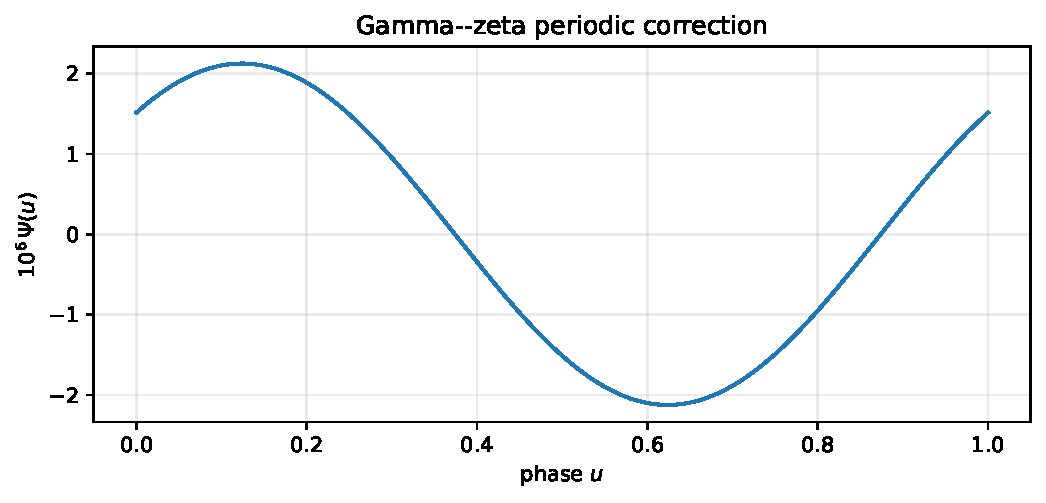
\includegraphics[width=0.82\textwidth]{psi_periodic.pdf}
\caption{The centered periodic Gamma--zeta correction.  Its amplitude is small,
but it occurs at the same asymptotic order as the nonoscillatory constants and
therefore cannot be dropped.}
\label{fig:psi}
\end{figure}

\begin{figure}[H]
\centering
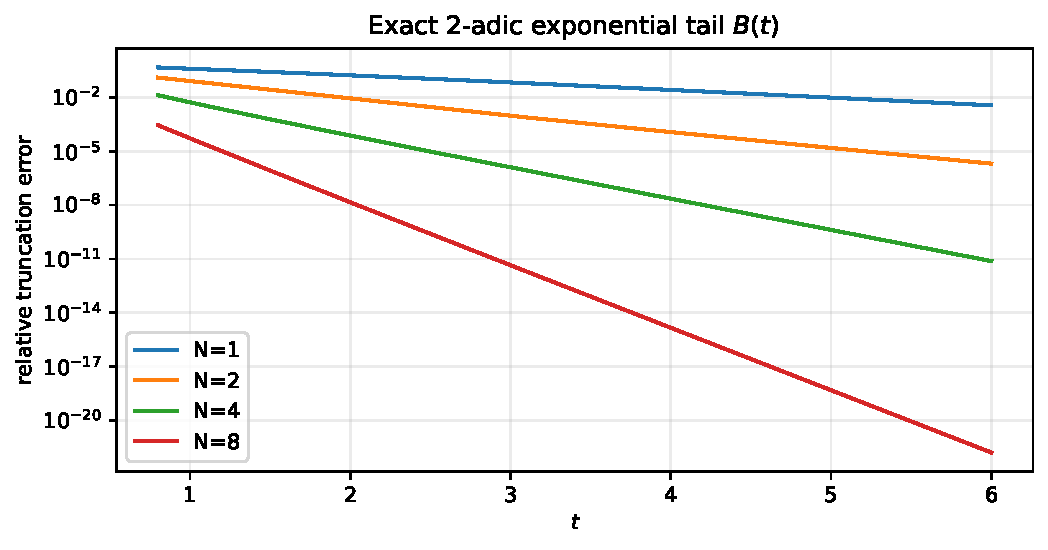
\includegraphics[width=0.82\textwidth]{dyadic_tail_convergence.pdf}
\caption{Relative error after retaining $N=1,2,4,8$ terms of the exact
$2$-adic exponential series for $B(t)$.  The bound
\eqref{eq:B-tail-bound} gives a simple rigorous enclosure.}
\label{fig:B-convergence}
\end{figure}

\section{Consequences and structural interpretation}
\label{sec:consequences}

\subsection{There is no phase-free complete expansion}

The first coefficient
\[
 g_1=\frac12\log\rho+\kappa_0-\Psi(\rho+\beta)
\]
already shows that a complete expansion cannot have constant coefficients in
powers of $\rho^{-1}$ and $\log\rho$ alone.  Formula \eqref{eq:dn-closed}
propagates phase derivatives to every later order.  The correct coefficient
ring is not $\R[\log\rho]$, but
\begin{equation}
 \R[\log\rho]\otimes
 C^\infty(\R/\Z)
 \label{eq:coefficient-ring}
\end{equation}
enlarged by the forward periodic saddle coefficients.  The phase circle is an
intrinsic asymptotic variable.

\subsection{Why the highest logarithms are nevertheless elementary}

Theorem \ref{thm:highest-log} shows a clean separation:
\begin{equation}
 \text{highest slow logarithm}
 \quad\text{is universal, while}\quad
 \text{phase information begins one degree lower}.
 \label{eq:separation}
\end{equation}
This reconciles two observations that can otherwise look contradictory.  An
elementary Lambert approximation captures the dominant logarithmic tower, but
it cannot be promoted to a complete asymptotic expansion because the periodic
coefficient at the next layer is nonconstant.

\subsection{A common Gamma--zeta source}

The denominator $1-2^{-s}$ has poles at the complex dimensions
$2\pi\ii k/L$.  In the small-$t$ Mellin expansion of $B$, they produce
$-\Psi$.  In the exact inverse expansion, derivatives and products of $\Psi$
are transported by Lagrange and Bell polynomials.  Thus the entire hierarchy
of inverse oscillations is generated from the same dyadic pole lattice; no new
frequencies are introduced, only integer convolutions of the existing modes.

\subsection{Arithmetic meaning of the ultraflat sectors}

The integer weight
\begin{equation}
 f(n):=nb_n=2^{\vTwo(n)+1}-1
 \label{eq:f-weight}
\end{equation}
counts the geometric sum of all dyadic representations $n=m2^k$.  It satisfies
\begin{equation}
 f(2n)=2f(n)+1,
 \qquad
 f(2n+1)=1.
 \label{eq:f-recursion}
\end{equation}
If $C(z)=\sum_{n\ge1}f(n)z^n$, then
\begin{equation}
 C(z)=2C(z^2)+\frac z{1-z}.
 \label{eq:C-Mahler}
\end{equation}
This puts the exponentially small saddle correction in the same digital
universe as the Thue--Morse and ruler sequences, but with a different
arithmetic statistic: geometric accumulation over the full $2$-adic valuation
rather than parity of the binary digit sum.

\section{Conjectures and research directions}
\label{sec:conjectures}

The following statements are deliberately separated from the proved results.
They are intended as concrete frontier problems rather than rhetorical
speculation.

\begin{conjecture}[Uniform Gevrey bound for phase-aware inverse coefficients]
\label{conj:Gevrey}
There exist constants $C,A>0$ and a phase-analytic strip
$\abs{\Im\phase}<\sigma$ such that the weighted analytic norms of the inverse
coefficients satisfy
\begin{equation}
 \norm{g_n}_{\sigma}\le CA^n n!
 \label{eq:Gevrey-bound}
\end{equation}
when the polynomial dependence on $\ell$ is measured with the natural weight
$1+\abs\ell$.  The same Gevrey order should hold for $d_n$ and $h_n$.
\end{conjecture}

A proof would require corresponding large-order control of the forward
$A_j$, followed by norm estimates for the closed Lagrange extractor.  The
finite formula \eqref{eq:dn-closed} is well suited to such estimates.

\begin{conjecture}[Sharp Fourier strip inheritance]
\label{conj:strip}
For every fixed $n$, each periodic coefficient of $d_n,h_n,g_n$ extends to the
same maximal horizontal strip as $\Psi$, and no generic cancellation enlarges
that strip.  In particular, the exponential rate of Fourier decay is stable
under all inverse coefficient operations.
\end{conjecture}

Differentiation, multiplication, and Bell composition preserve any smaller
strip.  The nontrivial part is sharpness: one must locate the nearest complex
singularities and exclude cancellation among the many differential-polynomial
terms.

\begin{conjecture}[Two-level exponentially improved inverse transseries]
\label{conj:hyper}
For $0<y\ll1$, let $q_\star(y)$ be the exact positive saddle coordinate defined
implicitly by
\begin{equation}
 G(y)=x\bigl(q_\star(y)\bigr),
 \label{eq:qstar-def}
\end{equation}
where $x(q)$ is the exact saddle map \eqref{eq:exact-saddle-map}.  After optimal
truncation of the algebraic phase-aware expansion, $G(y)$ admits an
exponentially improved description with at least two distinct levels:
ordinary saddle-resurgent sectors controlled by the large-order growth of the
$A_j$, and ultraflat dyadic sectors generated by
\begin{equation}
 \exp\bigl(-n2^{q_\star(y)}\bigr),
 \qquad n\ge1,
 \label{eq:ultraflat-scales}
\end{equation}
whose arithmetic seed is $b_n=(2^{\vTwo(n)+1}-1)/n$.
\end{conjecture}

The algebraic saddle inversion gives
$q_\star(y)=\phase+\bigO((\log\rho)/\rho)$, but this estimate does \emph{not}
permit replacing $q_\star$ by $\phase$ in \eqref{eq:ultraflat-scales}: the
induced change in the exponent is of order
$2^\phase(\log\rho)/\rho$, which diverges.  Thus the exact saddle coordinate is
part of the beyond-all-orders datum, not merely a cosmetic refinement.
Likewise, a naive substitution of \eqref{eq:B-2adic} into the ordinary saddle
series is not uniform because each derivative introduces powers of
$2^{q_\star}$; see \eqref{eq:B-Touchard}.  A correct theory likely needs an
accelerated or multilevel transseries in which $\rho^{-1}$ and
$\exp(-2^{q_\star(y)})$ are separate asymptotic monomials.

\begin{conjecture}[Resurgent arithmetic of the dyadic sectors]
\label{conj:resurgent-arithmetic}
Within the ultraflat level, the Stokes or connection coefficients are generated
by Dirichlet convolutions of the sequence $b_n$, so their Dirichlet series are
finite products of
\(
\zeta(s+1)/(1-2^{-s})
\)
and shifted variants.
\end{conjecture}

This is motivated by the fact that nonlinear saddle and inverse operations
multiply exponential sectors, turning coefficient sequences into additive
convolutions.  The conjecture is precise enough to test computationally once a
uniform hyperasymptotic construction is available.

\subsection{Promising concrete projects}

\begin{enumerate}
\item \textbf{Generate $A_2,A_3,A_4$ in compact Fourier-differential form.}
The partition formula \eqref{eq:Cn-partition} removes one combinatorial
bottleneck.  Combining it with the exact $q$-to-$\lambda$ conversion would make
$g_3,g_4,g_5$ completely explicit in $\Psi$ alone.

\item \textbf{Prove weighted Wiener-algebra bounds.}
Because the Fourier coefficients of $\Psi$ decay exponentially, a weighted
$\ell^1$ Fourier algebra should control products, derivatives, Lagrange
composition, and Bell polynomials uniformly in phase.

\item \textbf{Develop optimal truncation experiments.}
High-precision values of $G(y)$ can be compared with successive algebraic
truncations at fixed phase sequences.  The error should reveal whether the
first visible beyond-all-orders scale is saddle-resurgent or the much smaller
dyadic scale $\exp(-2^{q_\star(y)})$.

\item \textbf{Base-$b$ generalization.}
For a geometric scale $b^{-j}$, the analogue of \eqref{eq:B-2adic} is expected
to have coefficients
\[
 \frac{b^{\nu_b(n)+1}-1}{(b-1)n},
\]
and the same Dirichlet kernel $\zeta(s+1)/(1-b^{-s})$.  The resulting inverse
phase would have period one in $\log_b$.

\item \textbf{Lean formalization.}
The most modular targets are the generalized Lagrange formula
\eqref{eq:dn-closed}, the Bell extraction \eqref{eq:gn-direct}, the regrouping
proof of \eqref{eq:B-2adic}, and the Dirichlet identity
\eqref{eq:bn-dirichlet}.  Each can be formalized independently of delicate
contour estimates.
\end{enumerate}

\section{Formalization blueprint}
\label{sec:formalization}

A Lean development can be divided into four layers.

\begin{obligation}[Formal two-scale coefficient ring]
Define truncated series in $z$ with coefficients in a differential algebra of
polynomials in $\ell$ and smooth periodic functions of $\phase$.  Prove that
Taylor composition, inversion of $1+O(z)$, logarithm, and exponential preserve
truncation equivalence.
\end{obligation}

\begin{obligation}[Parameterized Lagrange inversion]
For a commutative $\Q$-algebra and $W=t\Phi(z,W)$, prove
\[
 [t^k]W=\frac1k[u^{k-1}]\Phi(z,u)^k.
\]
Specialize $t=z$ and prove \eqref{eq:dn-closed}.  This isolates the only
nontrivial formal-series theorem needed for the closed inverse coefficients.
\end{obligation}

\begin{obligation}[Gaussian contraction]
Represent a Gaussian moment functional algebraically by
$\E Z^{2m}=(2m-1)!!$ and $\E Z^{2m+1}=0$.  Expand
\eqref{eq:S-Gaussian} in a truncated graded algebra and prove the constrained
sum \eqref{eq:Cn-partition}.
\end{obligation}

\begin{obligation}[$2$-adic regrouping]
Formalize the bijection
\[
 \{(k,m):k\ge0,m\ge1,m2^k=n\}
 \longleftrightarrow
 \{0,1,\ldots,\vTwo(n)\}
\]
and sum the resulting geometric progression.  Absolute convergence then
justifies rearrangement in \eqref{eq:B-2adic}; a second Tonelli argument proves
\eqref{eq:bn-dirichlet}.
\end{obligation}

The contour-shift portion of \cref{thm:Mellin-bridge} is analytically deeper,
but it is not needed to formalize the exact arithmetic identities or the
closed inverse coefficient algebra.

\section{Conclusion}
\label{sec:conclusion}

The small-argument inverse Fabius function has a complete asymptotic expansion,
but its natural coefficient space is intrinsically two-scale.  The slow
variable is $\rho^{-1}\asymp(\log(1/y))^{-1/2}$, the slow logarithm is
$\log\rho$, and the fast variable is the exact phase
$\rho+1/\log2+1/2$ modulo one.  The repository had already established this
architecture and a recursive all-orders inversion.  The present report makes
the arbitrary-order coefficient genuinely explicit:
\begin{itemize}
\item generalized Lagrange--Bürmann gives $d_n$ directly;
\item partial Bell polynomials give $g_n$ directly;
\item the leading logarithm is universally $(\log\rho)^n/(2^nn!)$;
\item Gaussian contractions admit a finite constrained-partition formula;
\item inverse derivatives follow from one two-scale operator.
\end{itemize}

The exact dyadic Bose tail adds a second structural layer.  Its coefficients
are controlled by $\vTwo(n)$, its Mellin transform contains the same
Gamma--zeta complex dimensions as the periodic phase, and its derivative is
the exact exponentially small correction to the saddle map.  This turns a
formal ``beyond all orders'' remainder into an explicit arithmetic object and
provides a concrete route toward an exponentially improved inverse theory.

\appendix

\section{A compact coefficient dictionary}
\label{app:dictionary}

For convenient implementation, the full direct construction can be summarized
as follows:
\begin{align*}
 L&=\log2,
 &\beta&=L^{-1}+\tfrac12,
 &T&=\log(1/y),\\
 \rho&=\sqrt{2T/L},
 &z&=\rho^{-1},
 &\ell&=\log\rho,\\
 \phase&=\rho+\beta,
 &G_0&=\rho\e^{-L\rho-L\beta},
 &\lambda&=\rho+\beta+D,\\
 D&=\sum_{n\ge1}d_nz^n,
 &d_n&=\sum_{k=1}^n\frac{(-1)^k}{kL^k}
 [z^{n-k}u^{k-1}]\mathcal R^k,\\
 \frac{G}{G_0}&=(1+\beta z+zD)\e^{-LD},
 &g_n&=[z^n](1+\beta z+zD)\e^{-LD}.
\end{align*}
The residual $\mathcal R$ is given by \eqref{eq:R-functional}.  These lines
are sufficient to implement the complete inverse expansion once the forward
periodic coefficients $A_j$ are available.

\section{First generated saddle coefficients}
\label{app:generated}

For reference, the program generated the following logarithmic second saddle
coefficient:
\begin{align}
 \Lambda_2={}&\frac5{16}\rho_3^4+\frac58\rho_3^3
 -\frac{25}{48}\rho_3^2\rho_4+\frac98\rho_3^2
 -\frac23\rho_3\rho_4+\frac7{48}\rho_3\rho_5+2\rho_3
 \notag\\
 &+\frac1{12}\rho_4^2-\frac12\rho_4
 +\frac18\rho_5-\frac1{48}\rho_6+\frac52.
 \label{eq:Lambda2-expanded}
\end{align}
Higher generated expressions are archived separately rather than typeset in
full because their term count grows rapidly.

\section{Reproduction instructions}
\label{app:reproduction}

From the extracted archive directory, run
\begin{lstlisting}[language=bash]
python inverse_fabius_experiments.py --max-saddle-order 3
latexmk -pdf -interaction=nonstopmode -halt-on-error \
  inverse_fabius_complete_asymptotics.tex
\end{lstlisting}
The Python program regenerates
\path{generated_coefficients.tex}, \path{verification_output.txt}, and the two
vector PDF figures.  Increasing \texttt{--max-saddle-order} generates further
$C_n$ and $\Lambda_n$; symbolic size, rather than numerical instability, is
the main limitation.

\begin{thebibliography}{99}

\bibitem{RepoSnapshot}
V.~Reshetnikov,
\emph{ProveIt: Analysis/FabiusFunction documentation and Lean development},
Git repository snapshot
\texttt{ad82c27ffc6f90b3406f46c130c86d3cb83c6225}, 28 August 2026.

\bibitem{RepoInverse}
V.~Reshetnikov,
\emph{Inverse and Sampling Frontiers for the Fabius--Rvachev System},
\path{Analysis/FabiusFunction/docs/non-formalized-research-frontiers/drafts/inverse-and-sampling/Inverse_and_Sampling_Frontiers/Inverse_and_Sampling_Frontiers.tex},
2026.

\bibitem{RepoAudit}
V.~Reshetnikov,
\emph{Completion audit: corrected and full Fabius asymptotics},
\path{Analysis/FabiusFunction/docs/ASYMPTOTIC_COMPLETION_AUDIT.md}, 2026.

\bibitem{Fabius1966}
J.~Fabius,
A probabilistic example of a nowhere analytic $C^\infty$ function,
\emph{Zeitschrift f\"ur Wahrscheinlichkeitstheorie und Verwandte Gebiete}
\textbf{5} (1966), 173--174.

\bibitem{Corless}
R.~M.~Corless, G.~H.~Gonnet, D.~E.~G.~Hare, D.~J.~Jeffrey, and D.~E.~Knuth,
On the Lambert $W$ function,
\emph{Advances in Computational Mathematics} \textbf{5} (1996), 329--359.

\bibitem{Comtet}
L.~Comtet,
\emph{Advanced Combinatorics},
Reidel, 1974.

\bibitem{GouldenJackson}
I.~P.~Goulden and D.~M.~Jackson,
\emph{Combinatorial Enumeration},
Wiley, 1983.

\bibitem{FlajoletSedgewick}
P.~Flajolet and R.~Sedgewick,
\emph{Analytic Combinatorics},
Cambridge University Press, 2009.

\bibitem{deBruijn}
N.~G.~de Bruijn,
\emph{Asymptotic Methods in Analysis},
Dover, 1981.

\bibitem{Olver}
F.~W.~J.~Olver,
\emph{Asymptotics and Special Functions},
AKP Classics, 1997.

\bibitem{Wong}
R.~Wong,
\emph{Asymptotic Approximations of Integrals},
SIAM, 2001.

\bibitem{ParisKaminski}
R.~B.~Paris and D.~Kaminski,
\emph{Asymptotics and Mellin--Barnes Integrals},
Cambridge University Press, 2001.

\bibitem{Titchmarsh}
E.~C.~Titchmarsh,
\emph{The Theory of the Riemann Zeta-Function}, 2nd ed.,
revised by D.~R.~Heath-Brown, Oxford University Press, 1986.

\end{thebibliography}

\end{document}
